\chapter{Méthodologie}

\section{Introduction}

Dans cette partie de ce travail, nous allons nous intéresser tout particulièrement aux techniques mises en œuvre afin de résoudre notre type de problème. Nous commencerons par expliquer la manière dont nous avons perçu le problème, nous aborderons ensuite les diverses manières qui ont été proposées pour résoudre cette question. Et enfin, nous présenterons la solution que nous avons développée, ses tenants et aboutissants ainsi que les divers choix que nous avons dûs effectuer.

Nous vous le rappelons, notre problématique consiste, sur la base d'une liste d'ingrédients définie par l'utilisateur, d'en proposer d'autres qui sont gustativement associés. Un exemple serait que sur la base des mots "poulet" et "curry", notre algorithme nous propose du "riz". Il faut pour effectuer cette action, être capable d'associer des ensembles de mots ou \textit{ingrédients}, sur la base de concepts ou \textit{recettes}. Mais avant de voir comment nous pouvons parvenir à de tels résultats, nous allons faire un rappel des principes sous-jacents.

\section{Modèle vectoriel}

\subsection{Modèle}

La manière d'associer des concepts ensemble ou de rechercher des informations sont intrinsèquement liées. En effet, la recherche d'information $^{[2.2.3]}$ a pour objectif de trouver de manière performante une information perdue dans un vaste ensemble, souvent appelé \textit{corpus}. Ce corpus peut être très large ou contenir des informations de nature très variée et il peut donc être nécessaire d'avoir un retour de la part de l'utilisateur sur la pertinence de la réponse envoyée, afin de potentiellement mieux réorienter la recherche ou de simplement d'améliorer les résultats futurs.

Nous pouvons faire le parallèle avec la "vie réelle", en considérant le cas de la recherche d'un livre dans une bibliothèque. Imaginons, que vous soyez très intéressés par les populations, vous vous dirigerez de manière naturelle vers les rayonnages d'anthropologie, sachant pertinemment que votre recherche est bien vague. Mais si vous vous vouez de passion pour les indigènes d'Amazonie, alors vous aurez une bien plus grande précision dans votre démarche et chercherez le livre aux confluents de l'anthropologie et de l'Amazonie. Seulement, vous imaginez bien que ce système a des "failles" et que certains résultats, qui pourraient vous intéresser, se trouvent ailleurs, en mathématiques par exemple \cite{levi1949structures}. Il semble également évident que certains mots ont un poids beaucoup plus important et fournissent davantage de renseignements que d'autres. Il faut donc mieux orienter la recherche vers ces mots remplis de sens tout en respectant la volonté générale de la demande.

Une approche purement ensembliste et binaire n'est pas suffisante. Il nous faut définir un nouveau modèle qui nous permettra de trouver des réponses pertinentes aux requêtes, et ce, quelque soit la demande. Il peut donc être nécessaire d'observer un haut niveau d'abstraction. Bien sûr, pour pouvoir traiter nos informations, nous devrons mettre en place un formalisme afin de définir avec exactitude le contenu de notre corpus. Se poser des questions sur la nature même de ces objets, afin de mieux guider nos choix de représentations et ainsi avoir une plus grande appréciation sur la pertinence.

Ainsi, dans le domaine de l'informatique, les modèles nous aident à apporter un cadre déterminé et logique. Ils visent également à supporter notre intuition lors de la description de notre problématique. Ils servent d'abstraction et permettent de mettre en place toutes les propriétés mathématiques que nous pourrons employer. En l'occurrence, notre modèle servira à définir la représentation que prendront les documents du corpus, les requêtes et la notion de pertinence entre une demande et un résultat éventuel.

Mais comment élabore-t-on un modèle ? Il n'y a pas de réponses absolues, en ce sens que rien n'est jamais figé. Des découvertes ou des raisons techniques poussent à les faire évoluer, ils se peaufinent peu à peu avec le temps et les retours des utilisateurs. Comme les problèmes sont souvent mal définis, il reste une part de choix dans les paramètres qui constituent notre modèle et ceux-ci obtiennent une valeur souvent de manière empirique pour aboutir à des résultats toujours meilleurs. Par la suite, nous présenterons un modèle, parmi d'autres, qui est relativement commode à étudier et largement utilisé à travers la communauté informatique.

\subsection{Modèle vectoriel}

Énormément de modèles sont issus de diverses observations de la nature et le modèle vectoriel n'échappe pas à cette règle. L'idée est relativement simple, et permet une représentation aisée graphiquement. Cela a l'avantage de nous permettre de trouver plus facilement des liens, et de pouvoir disposer des outils proposés par la géométrie afin de mieux étudier ces corrélations.

On associe généralement le modèle vectoriel, avec son application aux données de type texte, aux travaux fournis dans les années 70 par Gerard Salton avec notamment son article \textit{A Vector Space Model for Automatic Indexing} (1975) \cite{Salton1975} et ses ouvrages sur le sujet qui restent encore toujours des références actuellement: \textit{Introduction to Modern Information Retrieval} (1983) \cite{salton1986introduction} ou \textit{Automatic Text Processing} (1989) \cite{salton1989automatic}.

Le principe de base de ce modèle est qu'on peut assimiler un document à une suite de termes appartenant au lexique d'une langue. En algèbre linéaire, chacun des mots de ce lexique correspondrait à un vecteur de base d'un espace vectoriel. Un exemple serait la phrase: "Plus blanc que blanc" qui pourrait se représenter mathématiquement par $1 * plus + 2 * blanc + 1 * que$. Ainsi, par cette application, nous pouvons faire correspondre nos documents à des vecteurs dont la dimension est égale à la taille du lexique. Il faut également avoir en tête que, de fait, le vecteur est épars, en ce sens qu'un document ne contient qu'une petite partie d'un corpus de mots, beaucoup de composantes valent zéro.

\begin{figure}[h]
\begin{center}
  \centering
    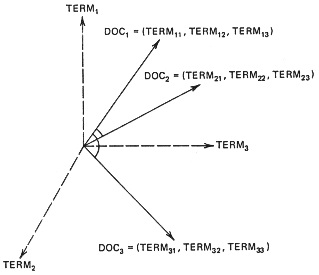
\includegraphics[scale=0.75]{Methodologie/vspace.jpg}
    \caption{Modèle vectoriel avec trois termes - tiré de Salton}
\end{center}
\end{figure}

\subsection{Similarité cosinus}

Cette représentation est relativement agréable mais ne nous permet pas encore de définir les documents les plus adéquats pour une requête donnée. Nous allons ici supposer que la similarité entre deux documents est simplement liée à la proximité de leur champ lexical et qu'une requête est un document par nature très court. Le problème revient à déterminer si le vecteur que représente notre requête nous envoie bien dans la bonne direction des résultats qui lui serait pertinente.

Nous pourrions estimer la pertinence d'un résultat comme sa distance par rapport au vecteur de demande, ainsi prendre une métrique qui lie les deux extrémités des vecteurs ou une notion qui va souvent de pair avec le concept même de distance, celui de la mesure de l'angle. Pour des raisons expliquées un peu plus loin, la distance $L_2$ (ou euclidienne) a moins de sens que la similarité cosinus et, on privilégie l'emploi de cette dernière. Nous pouvons caractériser la similarité entre deux documents comme étant l'angle formé entre le vecteur de requête et celui du document. Plus l'angle entre les deux est faible, plus les documents sont analogues. Il suffit alors simplement d'appliquer la formule brute du cosinus (si les deux vecteurs ne sont pas nuls) et nous obtenons le taux de similarité \cite{tan2006introduction}.

$$ similarity(A, B)  = \frac{A \cdot B}{\lVert A \rVert \lVert B \rVert} = \frac{\sum\nolimits_{i=1}^n A_i \times B_i}{\sqrt{\sum\nolimits_{i=1}^n A_i^2} \times \sqrt{\sum\nolimits_{i=1}^n B_i^2}} $$

où $A_i$ et $B_i$ correspondent à la composante associée au terme $i$. Si ces poids sont strictement positifs, nous obtenons donc que plus la similarité est grande, plus ce terme tend vers $1$:

$$ 0 \leq similarity(A, B) \leq 1 $$

\subsection{Vous avez dit mesure ?}

Il existe à priori plusieurs moyens de quantifier le taux de similarité entre deux documents dans ce modèle, toute métrique pouvant répondre à ce problème. Seulement, le choix d'une peut avoir de grandes conséquences sur les résultats obtenus. Par exemple, si nous employons la similarité cosinus, la taille des vecteurs n'a absolument aucune importance puisque nous nous intéressons uniquement à l'angle formé entre ceux-ci. Alors
 que si nous avions employé une métrique de type $L_p$, nous n'aurions regardé les résultats que dans un "cercle". Dans les deux cas, il y a une perte d'information et celle-ci peut avoir plus ou moins d'impact sur les résultats, quitte à les biaiser totalement. En pratique, le nombre élevé de dimensions combiné avec celui de documents que l'on considérera pourrait occulter en partie ces effets locaux. Quoiqu'il en soit, il vaut mieux toujours réaliser des tests sur la pertinence \cite{hand2001principles}.

De manière générale, choisir une "bonne" mesure se fait de manière expérimentale avec, potentiellement, une étude statistique sur la qualité de ces résultats. Nous verrons comment vérifier les réponses obtenues et leurs qualités plus tard$^{[\ref{section:Test}]}$. Il faut également savoir qu'il existe plusieurs phénomènes dont il faut avoir conscience:
\begin{itemize}
  \item Lorsque le nombre de dimensions devient élevé, des phénomènes qui semblent ne pas exister à faible dimensionnalité commence à avoir un impact de plus en plus important: on parle du \textit{fléau de la dimensionnalité} ou \textit{curse of dimensionality} \cite{bellman1957dynamic}.
  \item Comment peut-on interpréter les différences de résultats entre les diverses méthodes ? Toujours rester critique sur les observations effectuées !
  \item Notre corpus est-il de qualité ? Est-ce que les objets fortement décrits sont-ils plus souvent favorisés ou bien le contraire ?
  \item Nos mesures sont-elles réellement cohérentes ? Nos techniques employées également ? Ont-elles une signification particulière et adaptée en accord avec nos données et notre idée de résultat ?
\end{itemize}

Bien sûr, en recherche d'information, la mode est d'utiliser la similarité cosinus parce qu'elle semble mieux convenir aux résultats espérés puisqu'elle ne dépend pas de la norme des vecteurs et retourne un résultat entre $0$ et $1$. La majorité des composantes qui apparaissent dans un document sont nulles dans un autre. Alors que les distances peuvent obtenir des grands nombres qui sont difficilement comparables et sont sensibles à la norme. Les composantes sont également élevées à une puissance et ont donc un poids bien plus grand. Les résultats empiriques semblent indiquer que la similarité cosinus serait, en effet, en moyenne plus pertinent que les méthodes sur base d'une métrique \cite{qian2004similarity}. A noter qu'il existe également des outils statistiques tels que les coefficients de corrélation \cite{strehl2000impact}.

\subsection{TF-IDF}

Nous venons de discuter des questions de similarité mais nous n'avons pas abordé un problème plus profond qu'est celui des poids des termes et des valeurs des composantes. Une bonne pondération est important puisque celle-ci détermine la direction générale de ce vecteur. S'ils sont mal orientés et reflètent donc mal la sémantique du document, alors le concept de similarité cosinus s'écroule. Vous accepterez l'idée que certains mots dans un corpus ont beaucoup plus de poids que d'autres. Il existe des mots donnant une idée vague d'un concept et ceux pointus correspondant à des petites variations sémantiques dans un domaine. Généralement, un mot générique apparaîtra dans beaucoup plus de textes que des mots relatifs à une spécialité. On peut donc estimer que l'importance d'un mot est liée à l'importance de ce mot dans la littérature de manière générale et de sa fréquence d'apparition dans un document. Classiquement, pour représenter ce concept, on utilise le modèle du \textit{TF-IDF}.

Le principe même du \textit{TF-IDF} nous vient de M. Salton \cite{salton1988term} et part du constat qu'il est peu judicieux de considérer uniquement la fréquence d'un mot lors du calcul de son poids, il le définit donc comme étant une combinaison de deux aspects.
\begin{itemize}
  \item La fréquence (\textbf{Term Frequency}) \cite{Luhn:1957:SAM:1661832.1661836} est le nombre d’occurrences du terme $t$ dans le document $d$ parmi l'ensemble des mots existants: $tf(t, d) = \frac{n_{t, d}}{N_d}$. Afin que les documents puissent être comparés malgré leur différence de taille ou la répétition excessive d'un même mot-clef, il est nécessaire d'introduire un facteur de normalisation. Ici, il s'agit simplement du rapport entre le nombre d'occurrences et le nombre de termes qui existe, il existe beaucoup d'autres formules possibles. Signalons également la loi de Zipf qui établit que la fréquence d'apparition d'un terme est proportionnelle à l'inverse de son rang \cite{zipf1932selected}.
  \item L'inverse de la fréquence (\textbf{Inverse Document Frequency}) \cite{Jones72astatistical} qui consiste à diviser le nombre total de documents présents dans le corpus par le nombre de documents contenant ce terme $t$ et d'en prendre le logarithme par exemple: $idf(t, D) = log \frac{|D|}{|{d \in D: t \in d}|} $. L'idée est de mesurer la rareté du terme, celui-ci aura alors un impact plus ou moins grand sur la recherche. Le logarithme évite que cette fréquence ne soit trop prépondérante. 
\end{itemize}

Le modèle \textit{TF-IDF} consiste donc à estimer le poids d'un terme $t$ qui n'est plus seulement dépendant du document $d$ étudié, mais bel et bien de l'ensemble du corpus $D$. Nous avons donc:

$$ tfidf(t, d, D) = tf(t,d) \times idf(t, D) $$

\section{Prétraitement et recherche}

\subsection{Une question de langue}

Une des difficultés rencontrées dans le domaine de la recherche d'information concerne le traitement de la langue. En effet, afin de mieux orienter les recherches, il peut être intéressant d'être capable de déterminer les fonctions des termes employés. Une analyse sémantique ou syntaxique peut améliorer la compréhension globale des demandes effectuées et donc mieux correspondre aux besoins des utilisateurs.

L'étude même de cet aspect de l'informatique est liée à un domaine fort large, le \textit{traitement automatique du langage naturel} ou \textit{Natural Language Processing}. Cette branche vise à étudier les possibilités de traduction automatique, de réalisation des résumés ou de détecter des émotions au travers de l'écrit \cite{manning1999foundations}. Ici, nous n'emploierons qu'une infime partie des techniques employées afin de mieux extraire les mots-clefs d'un texte.

\subsection{Les mots vides}

Il existe, dans les langues, ce qu'on appelle communément des \textit{mots vides}, qui possèdent très peu de sémantique par eux-mêmes. Par exemple: le, du, ce, avoir, être, ... Si nous pondérons les termes par la technique du \textit{TF-IDF}, nous savons que ceux-ci auront un impact très faible sur les recherches, le coefficient \textit{IDF} tendra, en effet, vers zéro. Pour des raisons de ressources mémoires ou de performances, il peut donc être envisageable de les supprimer directement lors de la formation du corpus. Une méthode efficace, pour générer une liste de ces mots, consiste à analyser un corpus qui a l'air analogue et de sélectionner les termes dont le coefficient \textit{IDF} est pratiquement nul. Attention, supprimer ces mots n'est pas sans danger. En effet, il existe des expressions qui ne sont composées que de celles-ci: "être ou ne pas être" ou "the who". On peut imaginer qu'un moteur de recherche soit suffisamment malin pour repérer des motifs qui se répètent et donc générer des exceptions par lui-même. Ou plus simplement, changer de technique en fonction du taux de mots vides présents dans la recherche \cite{tong2011locating}.

\subsection{Orthographe et conjugaison}

On attend d'un moteur de recherche qu'il soit insensible au genre des mots, à leur conjugaison ou à leur forme. Une méthode efficace mais certes brutale pour répondre à ce problème est le \textit{stemming} ou \textit{désuffixation}, qui consiste à convertir tous les mots vers leur radical associé. Il faut bien sûr veiller au traitement de mots analogues mais dont le sens diffère fortement : (tu) bois et (un) bois. On peut également veiller à supprimer toutes les notions d'accentuation. Ces algorithmes sont fortement dépendants de la langue étudiée: agglutinante ou flexionnelle, indo-européenne ou autre. On pourra citer l'algorithme de Levins \cite{lovins1968development}, de Porter \cite{doi:10.1108/eb046814} ou de Paice \cite{Paice:1996:MES:230789.230796} pour l'Anglais ou Carry \cite{paternostre2002carry} ou Flemm \cite{namer2000flemm} pour le français.

Lorsqu'on écrit avec un clavier, on commet souvent des erreurs de frappe. Il peut alors être intéressant de proposer une correction orthographique à l'utilisateur pour obtenir de meilleurs résultats. La méthode la plus employée pour répondre à cette problématique est d'utiliser un dictionnaire et de comparer les mots de la requête avec celui-ci. Pour cela, on peut employer la distance de Levenshtein \cite{1966SPhD...10..707L}, ou une variante où la proximité des touches du clavier ou la phonétique interviennent.

\subsection{Index inversé} \label{subsubsection:Index inversé}

L'idée de l'index inversé provient de deux constatations:
\begin{itemize}
  \item Premièrement, calculer les \textit{TF-IDF} de l'ensemble d'un corpus peut prendre du temps et la matrice résultant doit être complètement recalculée à chaque fois qu'un nouveau document est ajouté à cet ensemble.
  \item Deuxièmement, les requêtes contiennent un tout petit ensemble de mots en comparaison à celui du corpus. Calculer la similarité cosinus avec tous les documents prendrait trop de temps et ne servirait à pas grand chose puisqu'il est probable que la majorité ne possède même pas un des termes de la demande.
\end{itemize}

Pour palier à ces problèmes, on emploie un index inversé afin d'offrir à la fois une rapidité d'indexation pour les nouveaux documents mais également une recherche performante. L'idée consiste à ne s'intéresser qu'aux mots et non aux documents, d'où l'origine du mot "inversé", tout en offrant une représentation du contenu exploitable. Sa structure est relativement simple, nous avons d'une part, une liste contenant tous les documents et le moyen d'y accéder ainsi que la taille de celui-ci et d'autre part, un index où à chaque mot du dictionnaire est associé la liste des paires des documents et le nombre d'occurrences où le terme apparaît. L'avantage d'une telle représentation est que le calcul du \textit{IDF}, au logarithme près, consiste simplement à faire le quotient entre le nombre de documents et le nombre de fois où le terme apparaît, soit la taille de la liste associée au mot. Le \textit{TF} est également très simple puisque nous possédons la taille de chaque document et que le nombre de fois où le terme apparaît dans le corpus est repris dans la liste associée au mot. Enfin, vous conviendrez que l'ajout de documents est aisé \cite{zobel2006inverted}. Attention, lorsque cette structure de données devient vraiment trop importante, des problèmes peuvent survenir \cite{brin2012reprint}.

\section{Décomposition en valeurs singulières}

Nous avons vu dans le chapitre précédent différents concepts clefs permettant d'effectuer des recherches de manière relativement efficace. Seulement, même si ces techniques ont beaucoup de qualité, elles sont peu adaptées à la résolution d'un problème qui lui est analogue. En effet, nous avons construit, avec notre modèle, une représentation spatiale des documents où leur position est définie par le contenu et il existe donc des sous-régions de cet espace ayant une certaine sémantique. Seulement, comment peut-on faire pour trouver des associations entre les mots ? Comment trouver un document contenant le mot "bateau" à l'aide du mot-clef "navire" ?

Nous verrons dans ce chapitre, une méthode afin de parvenir à la recherche de mots fortement corrélés dans une langue. Il existe d'autres procédures comme la \textit{Principal Component Analysis} \cite{pearson1901liii} ou la \textit{Non-Negative Matrix Factorization} \cite{paatero1994positive}, mais celles-ci ne seront pas abordées. Nous ne présenterons que la décomposition en valeurs singulières avant d'attaquer l'analyse sémantique latente.

\subsection{Valeurs propres}

Dans le terme décomposition en valeurs singulières, nous entendons \textit{valeurs singulières}. Un petit rappel sur la nature de ces valeurs et leur lien avec les valeurs propres peut être nécessaire.

Le concept de vecteur propre est une notion algébrique s'appliquant à une application linéaire d'un espace dans lui-même (\textit{endomorphisme}). On représente généralement les transformations linéaires de l'espace par des matrices qui sont des applications linéaires. En effet, celles-ci transforment les vecteurs en conservant les propriétés d'addition et de colinéarité. Cette propriété implique que, si on a un vecteur w, somme de deux vecteurs u et v, alors l'image de w sera également la somme des images des vecteurs u et v.

\begin{itemize}
  \item On appelle vecteur propre, un vecteur qui conserve sa direction (à ne pas confondre avec le sens) après transformation. (1)
  \item Une valeur propre est associée à un vecteur et représente le facteur d'homothétie de cette transformation. (2)
  \item Un espace propre est le sous-espace vectoriel qui contient l'ensemble des vecteurs propres.
\end{itemize}

Mathématiquement:
Soit $E$ un espace vectoriel sur un groupe commutatif $\mathbb{K}$ et $M$ un endomorphisme de $E$, alors:

\begin{itemize}
  \item Le vecteur $x$ de $E$ non nul est dit vecteur propre de $u$ si et seulement si il existe un élément $\lambda$ de $\mathbb{K}$, tel que $M(x) = \lambda x$. (1)
  \item Le scalaire $\lambda$ de $\mathbb{K}$ est dit valeur propre de $u$ si et seulement si il existe un vecteur $x$ non nul de $E$ tel que $M(x) = \lambda x$. (2)
\end{itemize}

Attention, les valeurs propres et vecteurs propres ne sont pas toujours réels et peuvent avoir des multiplicités supérieures à 1.

\subsection{Valeurs singulières}

Cette présentation brève de ce vaste champ des mathématiques ayant été effectuée, nous allons présenter ce qui s'appelle les valeurs singulières de manière très synthétique:

Soit $M$, une matrice $m \times n$ dont les coefficients appartiennent à un corps $\mathbb{K}$:
On appelle valeur singulière de $M$ toute racine carrée d'une valeur propre de $M^{*}M$, autrement dit tout réel positif $\sigma$ tel qu'il existe un vecteur unitaire $u$ dans $\mathbb{K}^{m}$ et un vecteur unitaire $v$ dans $\mathbb{K}^{n}$ vérifiant:

$$ Mv = \sigma u ~~~~ \text{et} ~~~~ M^{*}u = \sigma v $$

On dit que $u$ est un vecteur singulier gauche et $v$, droit pour $\sigma$.

\subsection{Décomposition}

La décomposition en valeurs singulières est très ancienne, on l'associe généralement aux travaux de Beltrami et Jordan, qui ont été généralisés par Eckart et Young avec le théorème d'Autonne-Eckart-Young \cite{eckart1939principal}. Ce théorème dit qu'on peut toujours décomposer une matrice en ceci:

$$ M = U \Sigma V^{*} $$

avec:
\begin{itemize}
  \item $M$, une matrice $m \times n$ avec au plus $min(m, n)$ valeurs singulières distinctes.
  \item $U$, une matrice orthogonale de $\mathbb{K}^{m}$ avec les vecteurs gauches de $M$.
  \item $\Sigma$, une matrice diagonale qui reprend les valeurs singulières de $M$. Habituellement, ces valeurs sont ordonnées dans l'ordre décroissant.
  \item $V^{*}$, une matrice orthogonale de $\mathbb{K}^{n}$ avec les vecteurs droits de $M$.
\end{itemize}

\subsection{Réduction de la dimensionnalité}

Nous l'avons dit, des problèmes peuvent apparaître avec un nombre de dimensions élevé. Il peut alors être intéressant de réduire cette dimensionnalité. On note $\Sigma_{k}$ la matrice $\Sigma$ où on n'a conservé que les $k$ premières valeurs singulières.

$$ \Sigma_k =\left( \begin{array}{cccc|ccc}
   \sigma_1 & 0 & \cdots & 0 & 0 & \cdots & 0 \\
   0 & \sigma_2 & \ddots & \vdots & \vdots & & \vdots \\
   \vdots & \ddots & \ddots & 0 & \vdots & & \vdots \\
   0 & \cdots & 0 & \sigma_k & 0 & \cdots & 0 \\ \hline
   0 & \cdots & \cdots & 0 & 0 & \cdots & 0 \\
   \vdots & & & \vdots & \vdots & & \vdots \\
   0 & \cdots & \cdots & 0 & 0 & \cdots & 0
\end{array}\right) $$

Grâce au théorème de Eckart-Young \cite{eckart1936approximation}, $M_{k} = U \Sigma_{k} V^{T}$ est la meilleure approximation de rang $k$ de $M$ selon la norme de Frobenius ou de Hilbert-Schmidt \cite{horn1990norms}.

$$ \|A\|_F=\sqrt{\sum_{i=1}^m\sum_{j=1}^n |a_{ij}|^2}=\sqrt{\operatorname{trace}(A^{{}^*}A)}=\sqrt{\sum_{i=1}^{\min\{m,\,n\}} \sigma_i^2} $$

On supprime généralement les termes ayant peu d'influences. En règle général, on garde toutes les valeurs représentant 90\% de la trace de la matrice ou on ne garde qu'une petite centaine de valeurs singulières.

\begin{figure}[h]
\begin{center}
    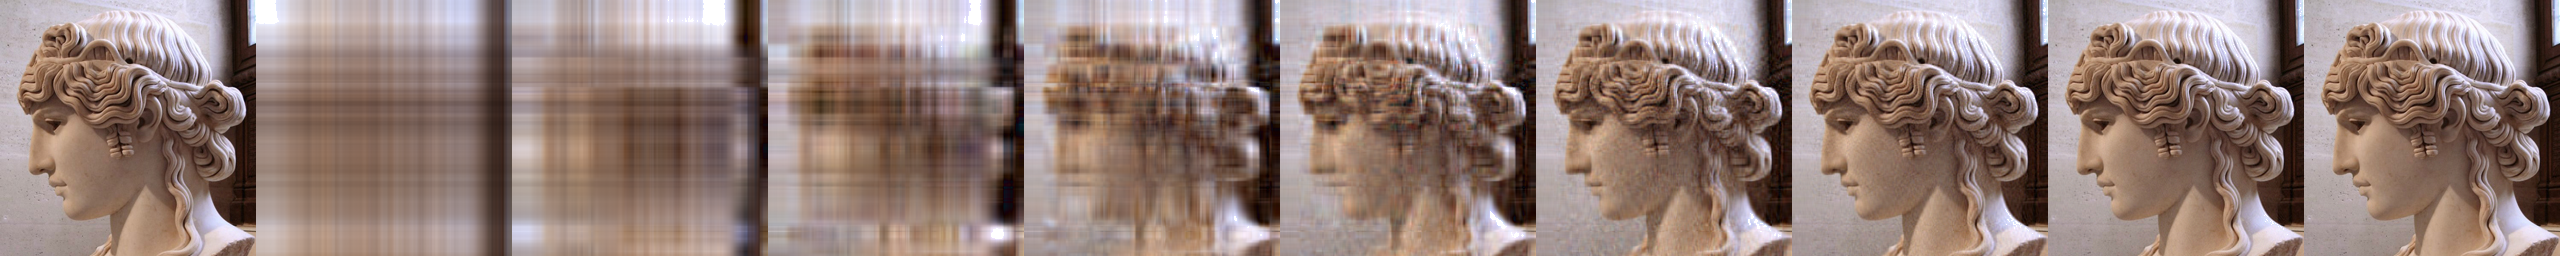
\includegraphics[scale=0.15]{Methodologie/Antinous_SVD_approximation.png}
    \caption{Approximations successives d'une image, avec 1, 2, 4, 8, 16, 32, 64, 128 puis toutes les valeurs singulières (image originale à gauche) - tiré de Wikimedia}
\end{center}
\end{figure}

\subsection{Interprétation géométrique}

Certains ont une vue plutôt algébrique et d'autres géométrique. Il est peut être avantageux de visualiser ce que représente ces matrices $U$, $\Sigma$ et $V^{*}$. Pour notre bien-être mental, nous allons nous cantonner à deux dimensions par la suite.

Si nous considérons une matrice $M$ carrée et dont le déterminant est positif, $U$ et $V^{*}$ représentent une rotation et $\Sigma$ une homothétie pour chacun des axes.

\begin{figure}[h]
\begin{center}
    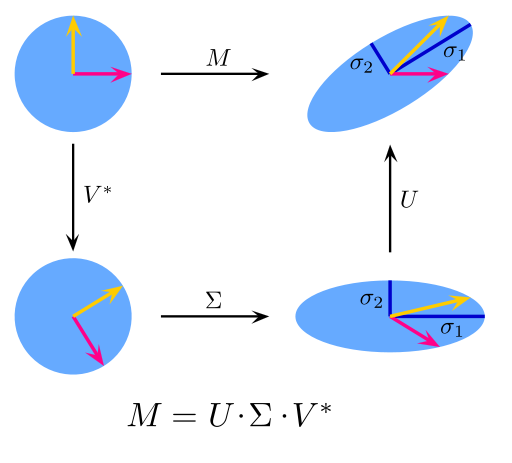
\includegraphics[scale=0.5]{Methodologie/Singular-Value-Decomposition.png}
    \caption{Transformation du cercle unité par la matrice (1 1, 0 1) - tiré de Wikimedia par Georg-Johann}
\end{center}
\end{figure}

La décomposition consiste à effectuer une rotation de l'espace à l'aide de la matrice $U$ afin de construire un nouvel espace orthogonal tel que la distance quadratique moyenne soit minimale par rapport à l'ensemble des points \cite{lawson1974solving}.

\begin{figure}[h]
\begin{center}
    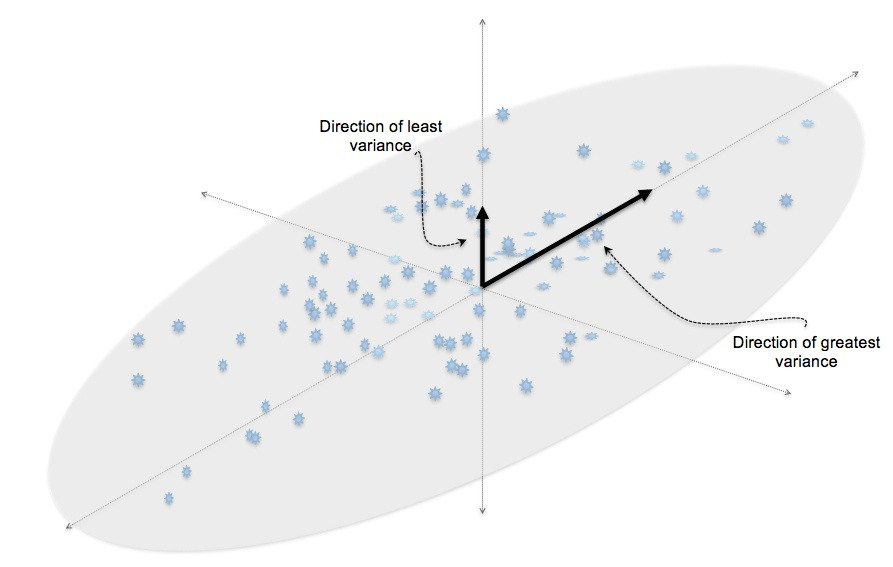
\includegraphics[scale=0.35]{Methodologie/main-qimg-fdce4658f6db6fa90ab42bff2ff81c61.jpg}
    \caption{Moindres carrés et orthogonalité - tiré de Mike Tamir}
\end{center}
\end{figure}

Et $V$, contient les nouvelles coordonnées dans la nouvelle base $U$. Conserver les premières valeurs singulières de $\Sigma$ permet de garder les axes qui contiennent la variance la plus forte, et donc le plus d'informations. À noter que pour obtenir la matrice nécessaire à la technique du \textit{PCA}, il suffirait de centrer la matrice au barycentre des données (ou centre de gravité pour les belges).

\section{Analyse sémantique latente}

La décomposition en valeurs singulières intervient dans plusieurs problèmes comme le calcul de matrice pseudo-inverse, la résolution de systèmes linéaires homogènes, les moindres-carrés, les matrices de rang inférieur, les modèles séparables ou encore dans le traitement du signal. Je vous invite à consulter la page Wikipédia pour obtenir encore plus d'informations sur ce sujet passionnant !

Mais cette décomposition intervient également pour un sujet qui va nous intéresser tout particulièrement, celui de l'analyse sémantique latente ou \textit{Latent Semantic Indexing/Analysis}. Qui consiste à identifier les liens qui unissent les termes aux concepts dans un ensemble non-structuré de textes. Le principe fondateur réside dans le fait que les mots employés dans un même contexte ont généralement un sens analogue. Tout aurait commencé grâce aux travaux de Jean-Paul Benzécri \cite{benzecri1976analyse} qui ont été améliorés par la société \textit{Bell Core} \cite{deerwester1989computer}. Dans cette partie, nous ne présenterons pas la technique dite du \textit{Probabilistic Latent Semantic Analysis} qui propose une approche purement statistique \cite{hofmann1999probabilistic}.

\subsection{Espace des concepts}

La matrice utilisée pour réaliser la décomposition en valeurs singulières est simplement une matrice qui contient l'occurrence du terme $t$ dans le document $d$. On peut également utiliser le poids du \textit{TF-IDF} pour chacun des termes. C'est généralement une matrice fort creuse, la majorité des termes étant égaux à zéro.

Lorsqu'on applique la décomposition en valeurs singulières, on crée une nouvelle base
 à partir des anciennes dimensions (les mots de notre corpus). Cette nouvelle base est obtenue par combinaison linéaire et on appelle communément la matrice $U$, la matrice des \textit{concepts}. La matrice $\Sigma$ reprend les taux de variations de ces concepts, les $k$ plus grandes valeurs permettant ainsi de "capturer" les dimensions qui possèdent le plus d'information et d'éliminer le bruit. $V$ aura peu d'importance pour la suite.

\subsection{Similarité des termes et des documents}

Il est possible de définir une matrice $U\Sigma$ (et $V\Sigma$) comme le produit matriciel de $U$ (resp. $V$) et $\Sigma$, nous les noterons par la suite $T$ et $D$. Ce choix est cohérent puisqu'il est facilement démontrable que $M^{*}M$ peut se simplifier avec une décomposition spectrale parce que une matrice orthogonale et sa transposée donne l'identité. Intuitivement, cela consiste à exagérer les concepts ayant beaucoup de poids afin de les rendre encore plus visibles.

Enfin il est intéressant de regarder le produit de $T^{T}T$ (et de $D^{T}D$), qui représentent les liens entre les différentes termes (et documents) deux à deux \cite{landauer1998introduction}.

\subsection{Requêtes dans l'espace}

Le calcul de la décomposition en valeurs singulières est une opération coûteuse, il peut alors être nécessaire de ne pas travailler avec l'ensemble de la base de données mais avec un sous-ensemble. L'autre partie étant alors convertie dans l'espace des concepts. Cette opération est analogue à la traduction d'une requête dans cet espace.

$$ \begin{matrix}
&Q=U\Sigma V_q^T \\
\Leftrightarrow &V_q^T = \Sigma^{-1}U^TQ \\
\Leftrightarrow &V_q\Sigma = Q^TU\Sigma^{-1}\Sigma
\end{matrix} $$



Avec $Q$, le vecteur de requête et $V_{q}$, la matrice orthogonale pour la requête. La projection de $Q$ sur l'espace réduit à $k$ dimensions s'obtient en calculant $V_{q}\Sigma_{k}$, ce qui revient à calculer les $k$ premières colonnes de $Q^{T}U$.

\begin{footnotesize}
\bibliographystyle{ieeetr}
\bibliography{Methodologie/bibliographyMethodology}
\end{footnotesize}